% Options for packages loaded elsewhere
% Options for packages loaded elsewhere
\PassOptionsToPackage{unicode}{hyperref}
\PassOptionsToPackage{hyphens}{url}
\PassOptionsToPackage{dvipsnames,svgnames,x11names}{xcolor}
%
\documentclass[
  letterpaper,
  DIV=11,
  numbers=noendperiod]{scrartcl}
\usepackage{xcolor}
\usepackage{amsmath,amssymb}
\setcounter{secnumdepth}{5}
\usepackage{iftex}
\ifPDFTeX
  \usepackage[T1]{fontenc}
  \usepackage[utf8]{inputenc}
  \usepackage{textcomp} % provide euro and other symbols
\else % if luatex or xetex
  \usepackage{unicode-math} % this also loads fontspec
  \defaultfontfeatures{Scale=MatchLowercase}
  \defaultfontfeatures[\rmfamily]{Ligatures=TeX,Scale=1}
\fi
\usepackage{lmodern}
\ifPDFTeX\else
  % xetex/luatex font selection
\fi
% Use upquote if available, for straight quotes in verbatim environments
\IfFileExists{upquote.sty}{\usepackage{upquote}}{}
\IfFileExists{microtype.sty}{% use microtype if available
  \usepackage[]{microtype}
  \UseMicrotypeSet[protrusion]{basicmath} % disable protrusion for tt fonts
}{}
\makeatletter
\@ifundefined{KOMAClassName}{% if non-KOMA class
  \IfFileExists{parskip.sty}{%
    \usepackage{parskip}
  }{% else
    \setlength{\parindent}{0pt}
    \setlength{\parskip}{6pt plus 2pt minus 1pt}}
}{% if KOMA class
  \KOMAoptions{parskip=half}}
\makeatother
% Make \paragraph and \subparagraph free-standing
\makeatletter
\ifx\paragraph\undefined\else
  \let\oldparagraph\paragraph
  \renewcommand{\paragraph}{
    \@ifstar
      \xxxParagraphStar
      \xxxParagraphNoStar
  }
  \newcommand{\xxxParagraphStar}[1]{\oldparagraph*{#1}\mbox{}}
  \newcommand{\xxxParagraphNoStar}[1]{\oldparagraph{#1}\mbox{}}
\fi
\ifx\subparagraph\undefined\else
  \let\oldsubparagraph\subparagraph
  \renewcommand{\subparagraph}{
    \@ifstar
      \xxxSubParagraphStar
      \xxxSubParagraphNoStar
  }
  \newcommand{\xxxSubParagraphStar}[1]{\oldsubparagraph*{#1}\mbox{}}
  \newcommand{\xxxSubParagraphNoStar}[1]{\oldsubparagraph{#1}\mbox{}}
\fi
\makeatother


\usepackage{longtable,booktabs,array}
\usepackage{calc} % for calculating minipage widths
% Correct order of tables after \paragraph or \subparagraph
\usepackage{etoolbox}
\makeatletter
\patchcmd\longtable{\par}{\if@noskipsec\mbox{}\fi\par}{}{}
\makeatother
% Allow footnotes in longtable head/foot
\IfFileExists{footnotehyper.sty}{\usepackage{footnotehyper}}{\usepackage{footnote}}
\makesavenoteenv{longtable}
\usepackage{graphicx}
\makeatletter
\newsavebox\pandoc@box
\newcommand*\pandocbounded[1]{% scales image to fit in text height/width
  \sbox\pandoc@box{#1}%
  \Gscale@div\@tempa{\textheight}{\dimexpr\ht\pandoc@box+\dp\pandoc@box\relax}%
  \Gscale@div\@tempb{\linewidth}{\wd\pandoc@box}%
  \ifdim\@tempb\p@<\@tempa\p@\let\@tempa\@tempb\fi% select the smaller of both
  \ifdim\@tempa\p@<\p@\scalebox{\@tempa}{\usebox\pandoc@box}%
  \else\usebox{\pandoc@box}%
  \fi%
}
% Set default figure placement to htbp
\def\fps@figure{htbp}
\makeatother

\ifLuaTeX
  \usepackage{luacolor}
  \usepackage[soul]{lua-ul}
\else
  \usepackage{soul}
\fi




\setlength{\emergencystretch}{3em} % prevent overfull lines

\providecommand{\tightlist}{%
  \setlength{\itemsep}{0pt}\setlength{\parskip}{0pt}}



 


\KOMAoption{captions}{tableheading}
\makeatletter
\@ifpackageloaded{caption}{}{\usepackage{caption}}
\AtBeginDocument{%
\ifdefined\contentsname
  \renewcommand*\contentsname{Table of contents}
\else
  \newcommand\contentsname{Table of contents}
\fi
\ifdefined\listfigurename
  \renewcommand*\listfigurename{List of Figures}
\else
  \newcommand\listfigurename{List of Figures}
\fi
\ifdefined\listtablename
  \renewcommand*\listtablename{List of Tables}
\else
  \newcommand\listtablename{List of Tables}
\fi
\ifdefined\figurename
  \renewcommand*\figurename{Figure}
\else
  \newcommand\figurename{Figure}
\fi
\ifdefined\tablename
  \renewcommand*\tablename{Table}
\else
  \newcommand\tablename{Table}
\fi
}
\@ifpackageloaded{float}{}{\usepackage{float}}
\floatstyle{ruled}
\@ifundefined{c@chapter}{\newfloat{codelisting}{h}{lop}}{\newfloat{codelisting}{h}{lop}[chapter]}
\floatname{codelisting}{Listing}
\newcommand*\listoflistings{\listof{codelisting}{List of Listings}}
\makeatother
\makeatletter
\makeatother
\makeatletter
\@ifpackageloaded{caption}{}{\usepackage{caption}}
\@ifpackageloaded{subcaption}{}{\usepackage{subcaption}}
\makeatother
\usepackage{bookmark}
\IfFileExists{xurl.sty}{\usepackage{xurl}}{} % add URL line breaks if available
\urlstyle{same}
\hypersetup{
  pdftitle={Welcome to Psych 101},
  colorlinks=true,
  linkcolor={blue},
  filecolor={Maroon},
  citecolor={Blue},
  urlcolor={Blue},
  pdfcreator={LaTeX via pandoc}}


\title{Welcome to Psych 101}
\author{}
\date{}
\begin{document}
\maketitle

\renewcommand*\contentsname{Table of contents}
{
\hypersetup{linkcolor=}
\setcounter{tocdepth}{3}
\tableofcontents
}

\subsection{Welcome to Psych 101}\label{welcome-to-psych-101}

\begin{itemize}
\tightlist
\item
  \href{https://docs.google.com/forms/d/e/1FAIpQLSdUFSyKnQBLoCZKxb9ZqzmwbEUo8gCqtwKAEaf-wJAfoVKlbA/viewform?usp=header}{\textbf{take
  this quick check-in survey : tinyurl.com/hifirstclass}}
\item
  \textbf{access these notes here} : tinyurl.com/welcome101class
\end{itemize}

\subsection{\texorpdfstring{\protect\pandocbounded{\includegraphics[keepaspectratio]{images/clipboard-3517259230.png}}}{}}\label{section}

\subsection{Announcements}\label{announcements}

\begin{itemize}
\tightlist
\item
  \textbf{Section Swap :} post on bCourses to find someone to swap with.
\item
  \textbf{Waitlisted Students :} Thanks for your patience! Go
  bears\ldots{}
\item
  \textbf{Join the Class Discord :} link on bCourses
\item
  \textbf{Next Week :}

  \begin{itemize}
  \tightlist
  \item
    Attend Discussion Section
  \item
    Read Chapter 1
  \item
    Complete Quiz 1
  \end{itemize}
\end{itemize}

\subsection{Agenda}\label{agenda}

\begin{itemize}
\item
  \textbf{10 Minutes :} Check-In
\item
  \textbf{45 Minutes :} Who and Why and What Statistics?
\item
  \textbf{10 Minutes :} Break Time
\item
  \textbf{45 Minutes :} Why R?
\end{itemize}

\section{Part 1 : Who and Why and What
Statistics?}\label{part-1-who-and-why-and-what-statistics}

\subsection{Who Statistics?}\label{who-statistics}

\subsubsection{Professor : Arman (Daniel)
Catterson}\label{professor-arman-daniel-catterson}

\begin{itemize}
\item
  \textbf{say :} Arman\ldots Professor\ldots Professor
  Catterson\ldots Dr.~Catterson
\item
  \textbf{from :} Austin, TX to UC Berkeley to stayin in the bay forever
  teaching here as an adjunct and full-time at Diablo Valley College.

  \begin{center}
  \includegraphics[width=4.40625in,height=\textheight,keepaspectratio]{lecture_images/0L_KermitBike.png}
  \end{center}
\end{itemize}

\subsubsection{Students : THIS CLASS IS FOR
Y'ALL!!!}\label{students-this-class-is-for-yall}

\begin{itemize}
\item
  attendance is critical, especially when you are behind.
\item
  your voice is needed.

  \begin{itemize}
  \item
    \href{https://journals.sagepub.com/doi/10.1177/1745691620927709}{\textbf{in
    psychology}} : majority of authors (and editors who control
    research) are white.
  \item
    \textbf{in the classroom :} we learn from each other.

    \begin{itemize}
    \item
      clap once if you are here\ldots.
    \item
      all talk at once~ :)
    \item
      look around the room
    \end{itemize}
  \end{itemize}
\end{itemize}

\pandocbounded{\includegraphics[keepaspectratio]{images/clipboard-505165644.png}}

\subsubsection{Buddy System}\label{buddy-system}

\begin{itemize}
\item
  everyone has a buddy
\item
  talk to your buddy in this class

  \begin{itemize}
  \item
    \textbf{ICE BREAKER :} Why did you sit in this seat on the first day
    of class? What went into that decision?
  \item
    \textbf{Why Psych 214?} Why are psych majors are REQUIRED to take a
    stats class??
  \end{itemize}
\end{itemize}

\subsection{Why Statistics?}\label{why-statistics}

\subsubsection{\texorpdfstring{\textbf{Statistics as a
language.}}{Statistics as a language.}}\label{statistics-as-a-language.}

\begin{itemize}
\tightlist
\item
  \textbf{What happens in a good language class?}
\end{itemize}

\subsubsection{\texorpdfstring{\textbf{Variables and
Variation.}}{Variables and Variation.}}\label{variables-and-variation.}

\begin{itemize}
\item
  \textbf{variation :} change, differences, growth, complexity

  \begin{itemize}
  \item
    \textbf{zero variation.} everyone is the same. :(
  \item
    \textbf{life is complex.} and statistics is about \emph{defining}
    that complexity
  \end{itemize}
\item
  \textbf{variable :} a thing that varies.
\end{itemize}

\href{https://www.monicacanilao.com/art/\#installation}{\begin{center}
\pandocbounded{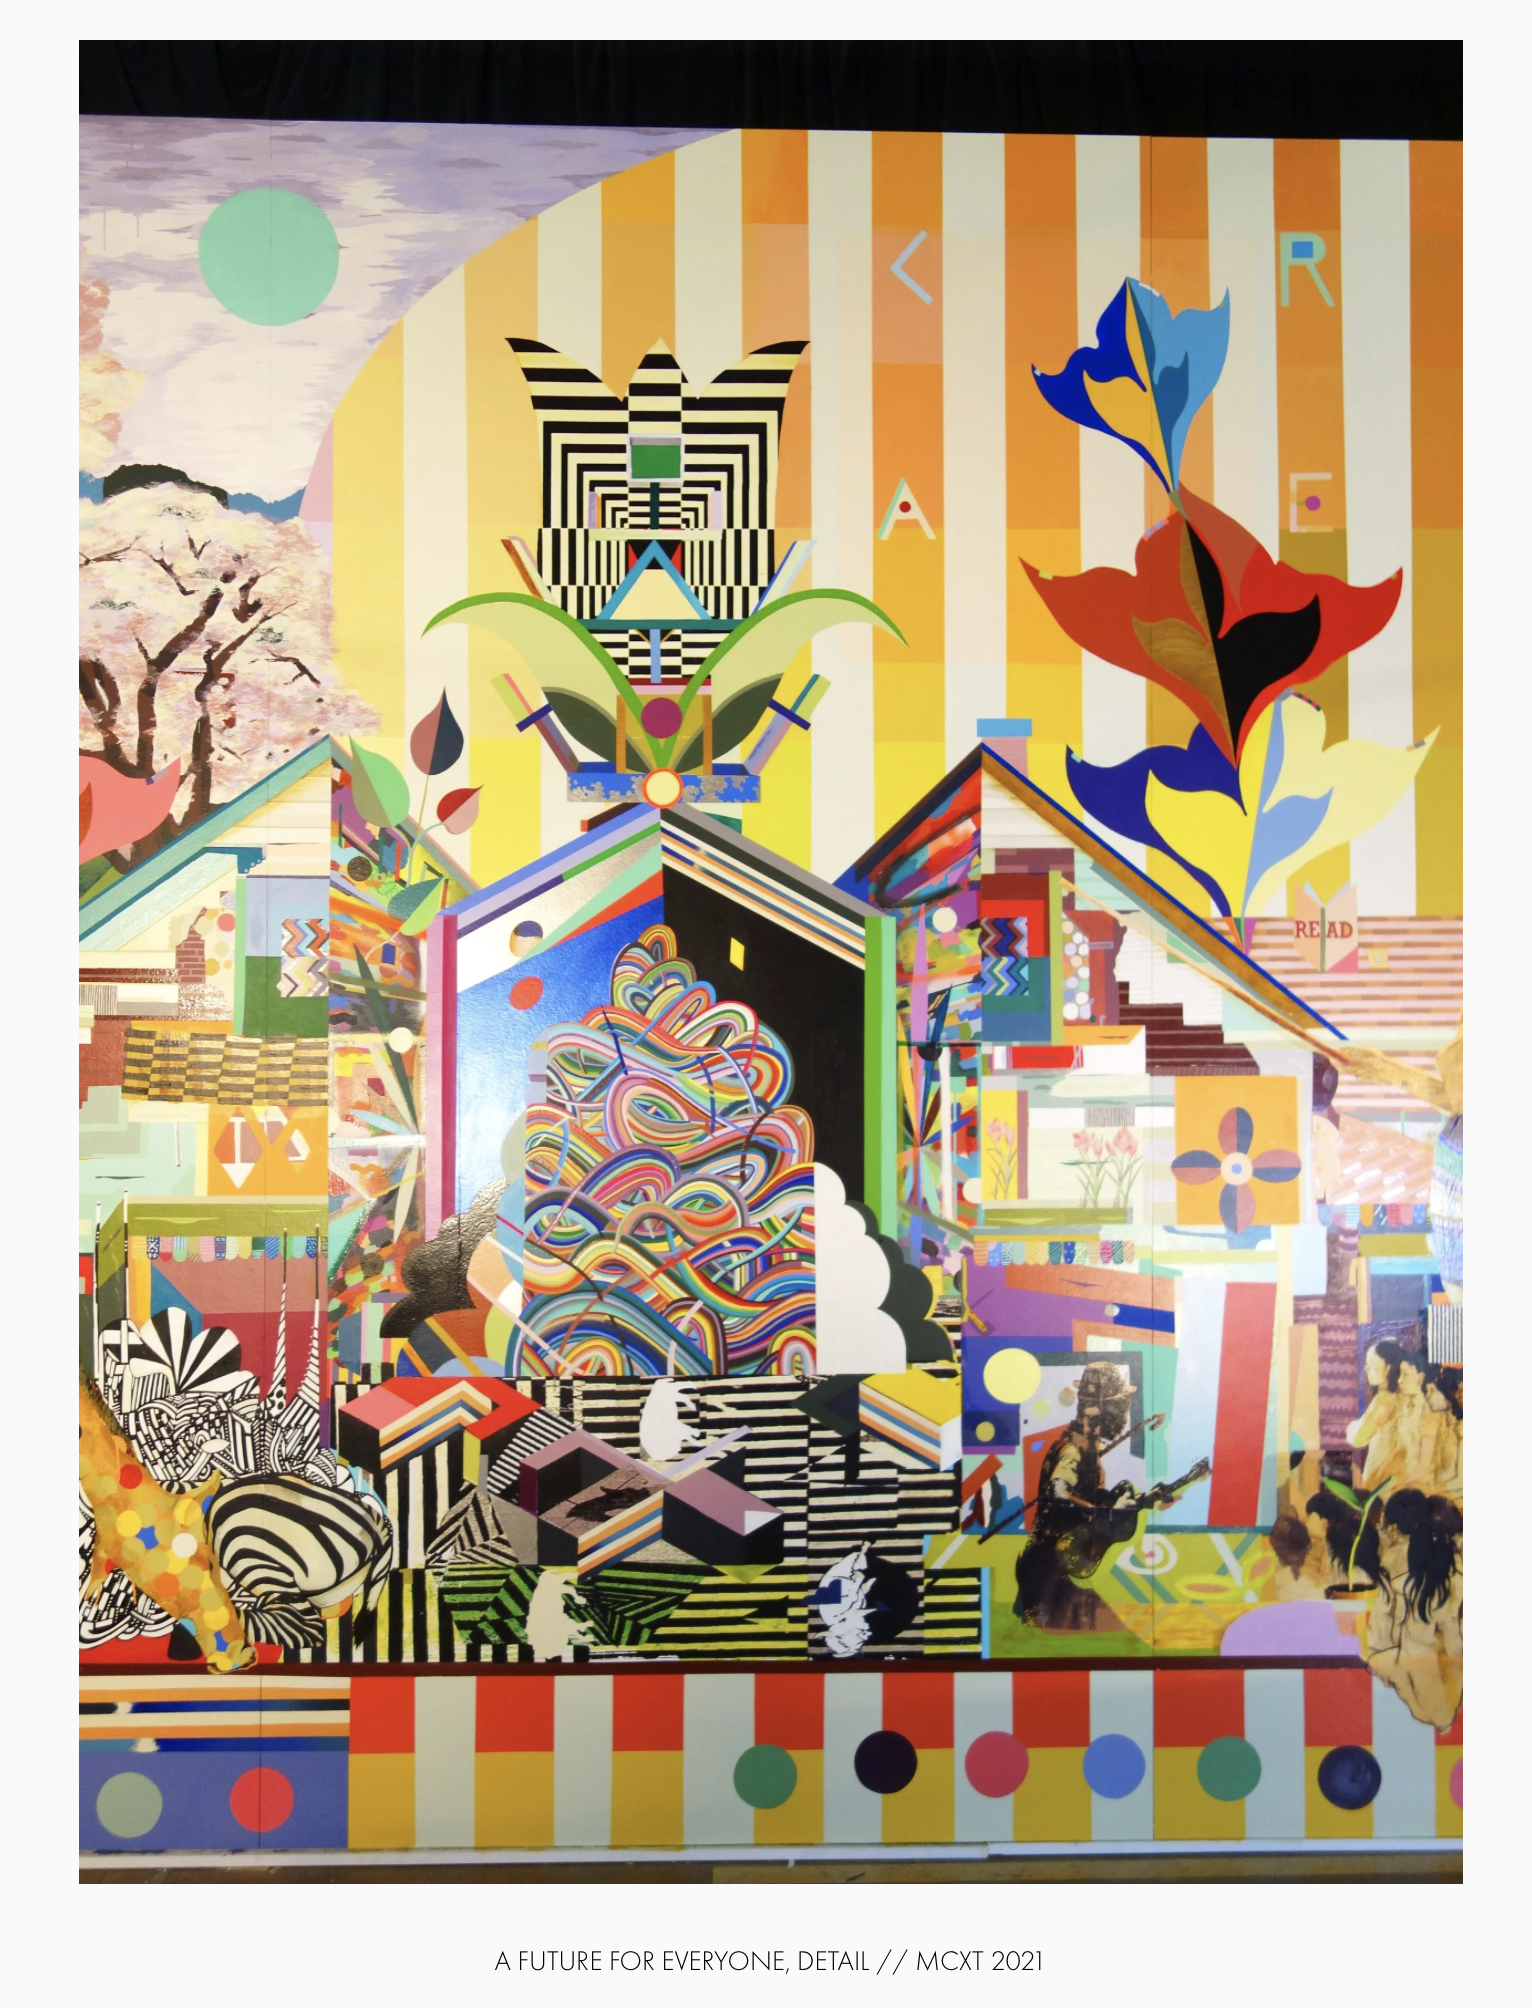
\includegraphics[keepaspectratio]{images/clipboard-1475096039.png}}
\end{center}
}

\subsubsection{\texorpdfstring{\textbf{the ABCs of
Psychology}}{the ABCs of Psychology}}\label{the-abcs-of-psychology}

\begin{itemize}
\item
  \textbf{Affect :} the emotions you feel
\item
  \textbf{Behavior :} the things you do
\item
  \textbf{Cognition :} the ideas (or brain activation) you think
\item
  \textbf{EXAMPLE : how can we think of happiness in terms of\ldots..}

  \begin{itemize}
  \item
    \textbf{Affect :}
  \item
    \textbf{Behavior :}
  \item
    \textbf{Cognition :}
  \end{itemize}
\end{itemize}

\subsubsection{\texorpdfstring{\textbf{Goal of
Science.}}{Goal of Science.}}\label{goal-of-science.}

\begin{itemize}
\item
  to describe variation
\item
  to make \ul{predictions} {[}see Chapter 1{]}
\end{itemize}

\begin{center}
\pandocbounded{\includegraphics[keepaspectratio]{lecture_images/0L_Halley.png}}
\end{center}

\subsection{What Statistics?}\label{what-statistics}

\subsubsection{This Semester}\label{this-semester}

\begin{itemize}
\item
  \textbf{Psych 101 :}

  \begin{itemize}
  \item
    \textbf{flipped classroom.} Readings before class; class time to
    practice and discuss.
  \item
    \textbf{We have a syllabus.} Any questions so far?
  \end{itemize}
\item
  \textbf{What \ul{predicts} a good class experience??}
\end{itemize}

\includegraphics[width=6.875in,height=\textheight,keepaspectratio]{images/clipboard-1054476114.png}

\subsubsection{Authentic Assessments}\label{authentic-assessments}

\begin{enumerate}
\def\labelenumi{\arabic{enumi}.}
\tightlist
\item
  \textbf{Brain Exams :} You look at some statistical results (graphs,
  tables) and interpret what you see with only your human brain to help
  you.
\item
  \textbf{R Exam :} You are given a dataset and a research question and
  asked to prepare a report with access to every possible tool you could
  want to use (see course AI policy).
\item
  \textbf{Final Project :} You learn more about a \ul{psychological
  variable} you care about, design a study to answer a question about
  this variable, collect the data from friends and family (n = 10),
  analyze the data using R, and write everything up as a research
  report.

  \begin{itemize}
  \tightlist
  \item
    \textbf{Milestone \#1 (in Section) :} What's a question you are
    interested in?
  \end{itemize}
\end{enumerate}

\subsubsection{AI Policy}\label{ai-policy}

\begin{itemize}
\item
  \textbf{AI as a tool} : you should be doing the learning.
\item
  \textbf{be transparent :} let us know how you used / share your
  prompts (see syllabus)
\item
  \textbf{imperfection is okay!} reach out for help if you are
  struggling.
\end{itemize}

\href{https://en.wikipedia.org/wiki/Ruth_Asawa}{\pandocbounded{\includegraphics[keepaspectratio]{images/clipboard-2700096382.png}}}

\section{BREAK TIME : MEET BACK AT
\_\_\_\_\_\_\_\_\_\_}\label{break-time-meet-back-at-__________}

\begin{center}
\pandocbounded{\includegraphics[keepaspectratio]{lecture_images/1L_breakhugme.avif}}
\end{center}

\section{Part 2 : Why R?}\label{part-2-why-r}

\subsection{Visualization Activity}\label{visualization-activity}

\begin{itemize}
\item
  Close your eyes
\item
  Take a deep breath (inhale / exhale)
\item
  Visualize an image based on the word that you hear me say.
\item
  What do you observe?
\end{itemize}

\subsection{Why R?}\label{why-r}

\begin{itemize}
\item
  \textbf{free :} open source, no cost,
\item
  \textbf{flexible :} can do many things (stats, graphs, authoring,
  works well with python tools)
\item
  \textbf{famous :} lots of tutorials, guides, courses, AI knows it,
  respected in psychology / sciences.
\end{itemize}

\subsection{R is Your New Friend}\label{r-is-your-new-friend}

\subsubsection{\texorpdfstring{\textbf{The R Console
:}}{The R Console :}}\label{the-r-console}

\begin{itemize}
\item
  where R does its work
\item
  what's your first reaction to this image? what does your eye look at?
  gloss over?
\end{itemize}

\begin{center}
\includegraphics[width=4.92708in,height=\textheight,keepaspectratio]{images/clipboard-4175992679.png}
\end{center}

\subsubsection{\texorpdfstring{\textbf{RStudio :} Integrated Development
Environment
(IDE)}{RStudio : Integrated Development Environment (IDE)}}\label{rstudio-integrated-development-environment-ide}

\begin{center}
\pandocbounded{\includegraphics[keepaspectratio]{images/clipboard-129412344.png}}
\end{center}

\subsection{Activities.}\label{activities.}

\begin{itemize}
\item
  Let's explore R (and when I say R, I mean to access \& open RStudio.)
\item
  Things to do :

  \begin{itemize}
  \item
    create a script.
  \item
    write a basic math problem that caused you trouble as a kid.
  \item
    teach R something (use the assign function)
  \item
    play around! it's okay to break things.
  \end{itemize}
\end{itemize}

\section{\texorpdfstring{\href{https://docs.google.com/forms/d/e/1FAIpQLSez8jfYb9hi5fAQsLj4LYEfql3qK1oxxJrtEXxdqDSDo5ha6g/viewform?usp=publish-editor}{Check-Out
:
tinyurl.com/byefirstclass}}{Check-Out : tinyurl.com/byefirstclass}}\label{check-out-tinyurl.combyefirstclass}




\end{document}
